%TEX root = ../dissertation.tex

\chapter{Pulsarcast}
\label{chapter:pulsarcast}

- Introduzir as decisões de arquitectura
  - Topic based subscriptions
  - Suporte para sub tópicos
  - Baseado num overlay estruturado (kadmelia DHT) para peer-discovery e
  storage, por cima do qual depois criamos o nosso "overlay"
  - Imutabilidade dos dados (tópicos e dados)
  - Nós guardam informação das msgs que recebem


\section{Data Structures}
- Introduzir conceito de event descriptor e topic descriptor
- Abordar imutabilidade mais a fundo
- JSON schema de ambos
- Representação com figuras
- Exemplos práticos?

\section{Subscription Management and Event Dissemination}
- Árvores de disseminação
  - Criação
  - Uso da DHT
  - Algoritmo em detalhe
- Disseminação de eventos


\begin{figure}[hb!]
  \centering
  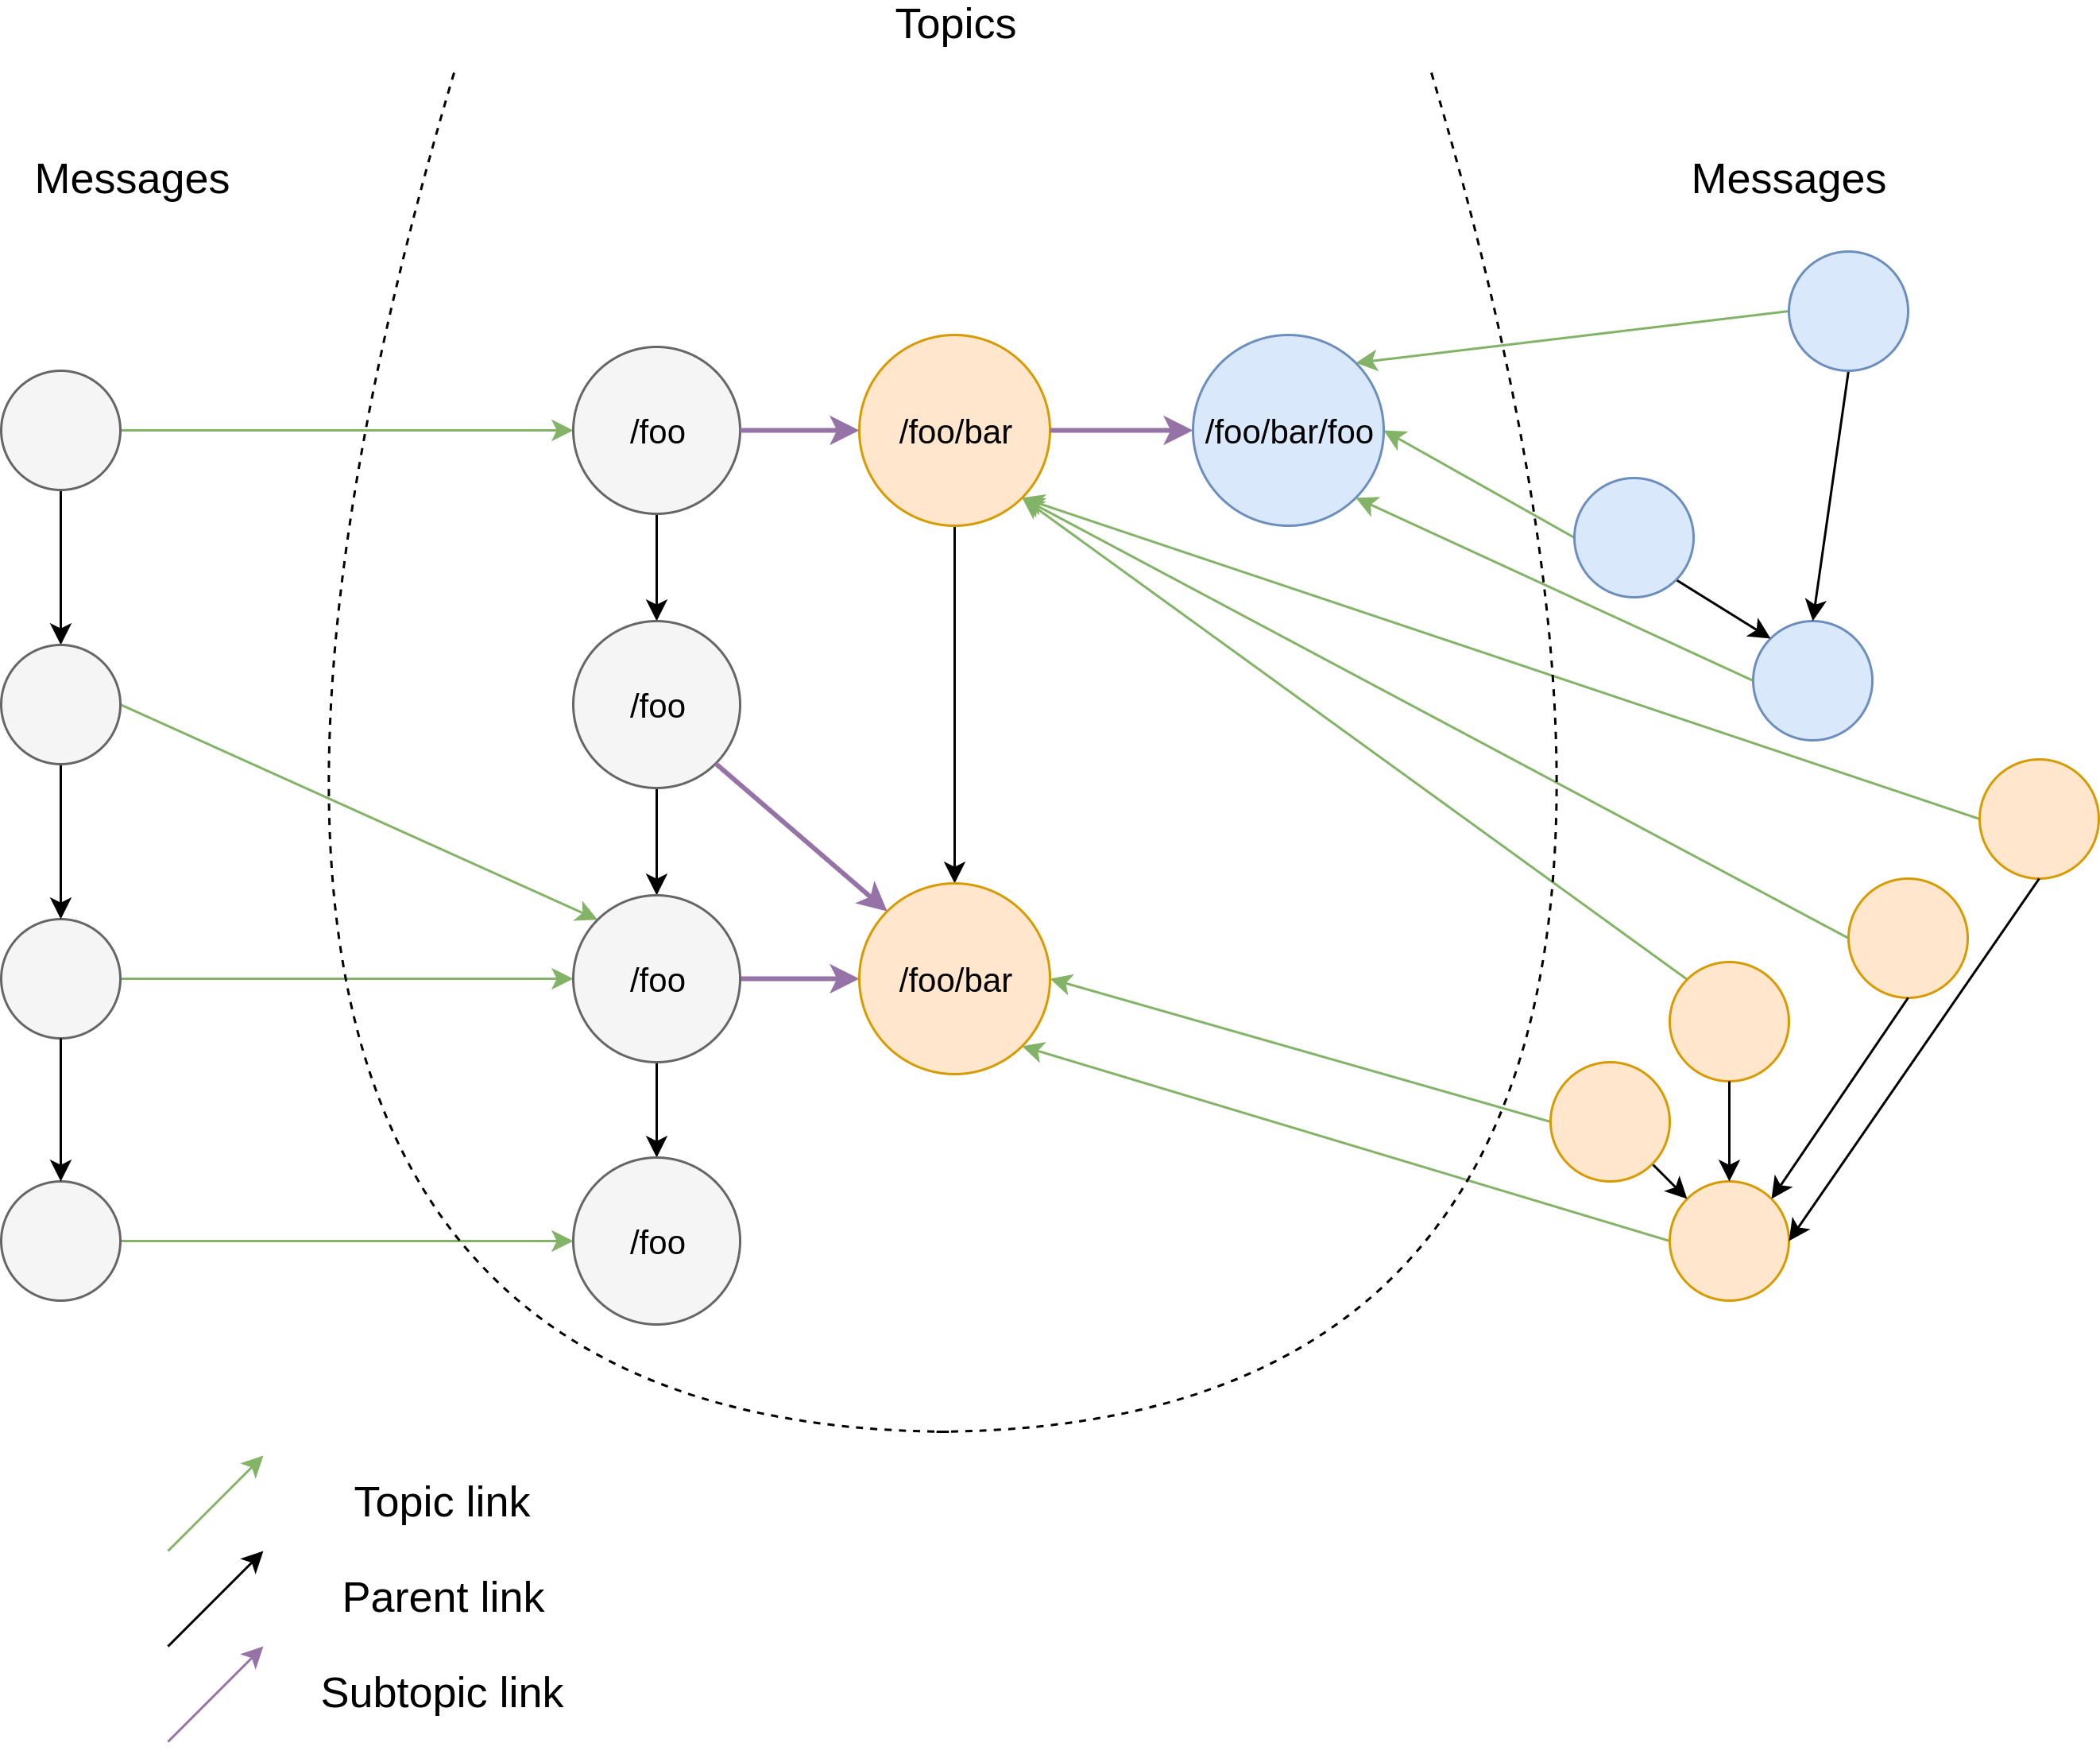
\includegraphics[width=0.95\textwidth]{img/pulsarcast-dag.png}
  \caption{Representation of the Pulsarcast DAG}
  \label{fig:pulsarcast-dag}
\end{figure}


\section{RPC Protocol}
